\documentclass[tikz,border=8pt]{standalone}
% Shared look for every TikZ diagram. Load with % Shared look for every TikZ diagram. Load with % Shared look for every TikZ diagram. Load with \input{../../tools/tikz-style.tex}
\usepackage[T1]{fontenc}
\usepackage{lmodern}
\renewcommand{\sfdefault}{lmr}  % diagrams use the same serif as the text
\usetikzlibrary{arrows.meta, positioning, shapes.geometric, calc, fit, backgrounds}
\definecolor{cblue}{HTML}{4C78A8}
\definecolor{corange}{HTML}{F58518}
\definecolor{cgreen}{HTML}{54A24B}
\definecolor{cred}{HTML}{E45756}
\definecolor{cpurple}{HTML}{B279A2}
\definecolor{cgrey}{HTML}{6B6B6B}
\tikzset{
  every picture/.style={font=\sffamily, line width=1.2pt},
  box/.style={draw=#1, fill=#1!12, rounded corners=4pt, align=center, inner sep=7pt, minimum height=1.1cm},
  box/.default=cgrey,
  arrow/.style={-{Stealth[length=3mm]}, draw=cgrey, line width=1.4pt},
  title/.style={font=\sffamily\bfseries\Large},
  note/.style={font=\sffamily\small, text=cgrey, align=center},
}
\AtBeginDocument{\hyphenpenalty=10000 \exhyphenpenalty=10000}

\usepackage[T1]{fontenc}
\usepackage{lmodern}
\renewcommand{\sfdefault}{lmr}  % diagrams use the same serif as the text
\usetikzlibrary{arrows.meta, positioning, shapes.geometric, calc, fit, backgrounds}
\definecolor{cblue}{HTML}{4C78A8}
\definecolor{corange}{HTML}{F58518}
\definecolor{cgreen}{HTML}{54A24B}
\definecolor{cred}{HTML}{E45756}
\definecolor{cpurple}{HTML}{B279A2}
\definecolor{cgrey}{HTML}{6B6B6B}
\tikzset{
  every picture/.style={font=\sffamily, line width=1.2pt},
  box/.style={draw=#1, fill=#1!12, rounded corners=4pt, align=center, inner sep=7pt, minimum height=1.1cm},
  box/.default=cgrey,
  arrow/.style={-{Stealth[length=3mm]}, draw=cgrey, line width=1.4pt},
  title/.style={font=\sffamily\bfseries\Large},
  note/.style={font=\sffamily\small, text=cgrey, align=center},
}
\AtBeginDocument{\hyphenpenalty=10000 \exhyphenpenalty=10000}

\usepackage[T1]{fontenc}
\usepackage{lmodern}
\renewcommand{\sfdefault}{lmr}  % diagrams use the same serif as the text
\usetikzlibrary{arrows.meta, positioning, shapes.geometric, calc, fit, backgrounds}
\definecolor{cblue}{HTML}{4C78A8}
\definecolor{corange}{HTML}{F58518}
\definecolor{cgreen}{HTML}{54A24B}
\definecolor{cred}{HTML}{E45756}
\definecolor{cpurple}{HTML}{B279A2}
\definecolor{cgrey}{HTML}{6B6B6B}
\tikzset{
  every picture/.style={font=\sffamily, line width=1.2pt},
  box/.style={draw=#1, fill=#1!12, rounded corners=4pt, align=center, inner sep=7pt, minimum height=1.1cm},
  box/.default=cgrey,
  arrow/.style={-{Stealth[length=3mm]}, draw=cgrey, line width=1.4pt},
  title/.style={font=\sffamily\bfseries\Large},
  note/.style={font=\sffamily\small, text=cgrey, align=center},
}
\AtBeginDocument{\hyphenpenalty=10000 \exhyphenpenalty=10000}

\begin{document}
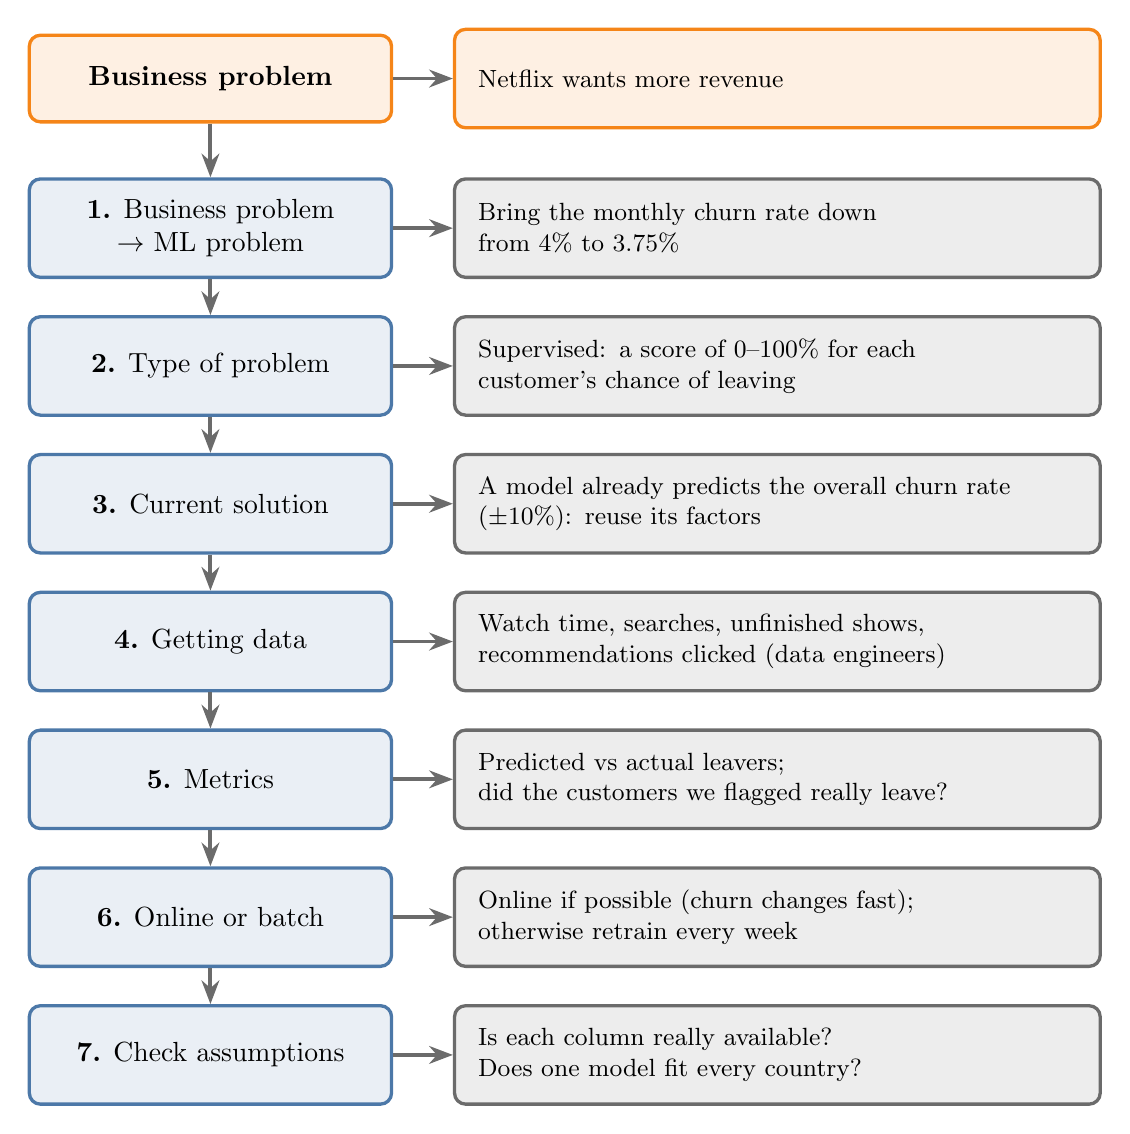
\begin{tikzpicture}
  \tikzset{
    stp/.style={box=cblue, minimum width=4.6cm, minimum height=1.25cm, font=\normalsize},
    ans/.style={box=cgrey, minimum width=8.2cm, minimum height=1.25cm, font=\small, align=left, text width=7.6cm},
  }
  \node[box=corange, minimum width=4.6cm, minimum height=1.1cm] (b) at (0,1.9) {\textbf{Business problem}};
  \node[ans, draw=corange, fill=corange!12] (ba) at (7.2,1.9) {Netflix wants more revenue};
  \draw[arrow] (b) -- (ba);
  \foreach \i/\s/\a in {
      1/{\textbf{1.} Business problem\\$\rightarrow$ ML problem}/{Bring the monthly churn rate down\\from 4\% to 3.75\%},
      2/{\textbf{2.} Type of problem}/{Supervised: a score of 0--100\% for each\\customer's chance of leaving},
      3/{\textbf{3.} Current solution}/{A model already predicts the overall churn rate\\($\pm$10\%): reuse its factors},
      4/{\textbf{4.} Getting data}/{Watch time, searches, unfinished shows,\\recommendations clicked (data engineers)},
      5/{\textbf{5.} Metrics}/{Predicted vs actual leavers;\\did the customers we flagged really leave?},
      6/{\textbf{6.} Online or batch}/{Online if possible (churn changes fast);\\otherwise retrain every week},
      7/{\textbf{7.} Check assumptions}/{Is each column really available?\\Does one model fit every country?}}
  {
    \node[stp] (s\i) at (0,-1.75*\i+1.75) {\s};
    \node[ans] (a\i) at (7.2,-1.75*\i+1.75) {\a};
    \draw[arrow] (s\i) -- (a\i);
  }
  \draw[arrow] (b) -- (s1);
  \foreach \a/\b in {1/2, 2/3, 3/4, 4/5, 5/6, 6/7} \draw[arrow] (s\a) -- (s\b);
\end{tikzpicture}
\end{document}
